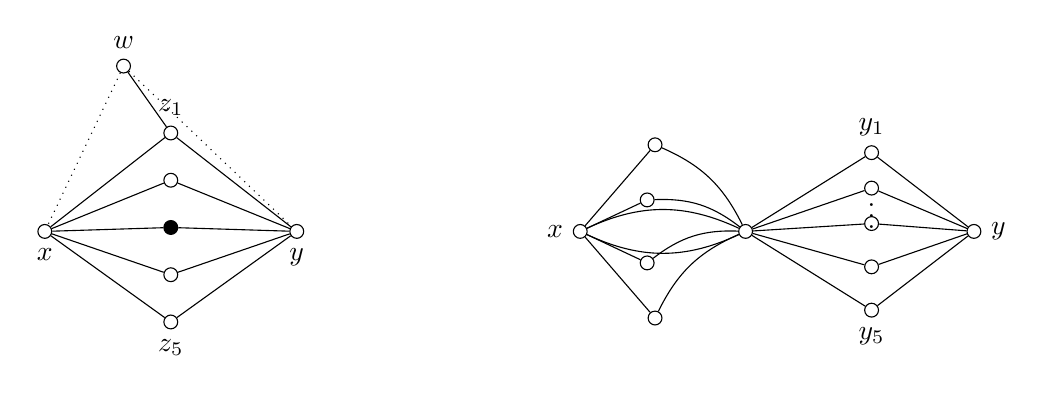
\begin{tikzpicture}[
  v/.style={circle,draw,fill=white,inner sep=0pt,minimum size=5pt},
  vf/.style={circle,draw,fill=black,inner sep=0pt,minimum size=5pt}
]

%-----------------------------------
% Left: The case S ⊄ N[x] ∪ N[y] and |Z| ≥ 5
%-----------------------------------
\begin{scope}
  % base vertices
  \node[v,label=below:$x$] (x) at (0,0) {};
  \node[v,label=below:$y$] (y) at (3.2,0) {};

  % Z column (five vertices, middle one filled)
  \node[v,label=above:$z_1$] (z1) at (1.6,1.25) {};
  \node[v] (z2) at (1.6,0.65) {};
  \node[vf] (z3) at (1.6,0.05) {};
  \node[v] (z4) at (1.6,-0.55) {};
  \node[v,label=below:$z_5$] (z5) at (1.6,-1.15) {};

  % Edges from x and y to each z_i
  \foreach \z in {z1,z2,z3,z4,z5}{
    \draw (x) -- (\z);
    \draw (y) -- (\z);
  }

  % A vertex w ∈ S \ (N[x] ∪ N[y])
  \node[v,label=above:$w$] (w) at (1.0,2.1) {};
  \draw[dotted] (w) -- (x);
  \draw[dotted] (w) -- (y);
  \draw (w) -- (z1);
\end{scope}

%-----------------------------------
% Right: Proof of Claim ~\ref{clm3}, assuming ∃ x_i with |N(x_i)∩Y| ≥ 5
%-----------------------------------
\begin{scope}[xshift=6.8cm]
  % endpoints
  \node[v,label=left:$x$] (xr) at (0,0) {};
  \node[v,label=right:$y$] (yr) at (5.0,0) {};

  % the special vertex x_i in the middle (left unlabeled as in the figure)
  \node[v] (xi) at (2.1,0) {};

  % left fan toward x (four auxiliary vertices forming a fan into x_i)
  \node[v] (l1) at (0.95,1.10) {};
  \node[v] (l2) at (0.85,0.40) {};
  \node[v] (l3) at (0.85,-0.40) {};
  \node[v] (l4) at (0.95,-1.10) {};
  \foreach \l in {l1,l2,l3,l4}{
    \draw (xr) -- (\l);
    \draw[bend left=20] (\l) to (xi);
  }

  % Y-neighbors of x_i (at least five)
  \node[v,label=above:$y_1$] (y1) at (3.7,1.00) {};
  \node[v] (y2) at (3.7,0.55) {};
  \node[v] (y3) at (3.7,0.10) {};
  \node[v] (y4) at (3.7,-0.45) {};
  \node[v,label=below:$y_5$] (y5) at (3.7,-1.00) {};

  % Connect x_i to these Y vertices, and each to y (triangular fan near y)
  \foreach \yy in {y1,y2,y3,y4,y5}{
    \draw (xi) -- (\yy);
    \draw (\yy) -- (yr);
  }

  % a couple of parallel curved connections x -- x_i (as in the figure’s styling)
  \draw[bend left=25]  (xr) to (xi);
  \draw[bend right=25] (xr) to (xi);

  % vertical ellipsis indicating many Y-vertices
  \node at (3.7,0.30) {$\vdots$};
\end{scope}

\end{tikzpicture}